% ----------------------------------------------------------------
% DUMMY PAPER USING MANUSCRIPT_MODERN CLASS
% ----------------------------------------------------------------
\documentclass{manuscript_modern}
\usepackage{lipsum}
\usepackage{graphicx}
\usepackage{mwe} % for placeholder images

% Default bibliography using biblatex is assumed. You can override:
% \usepackage[style=nature]{biblatex}
\addbibresource{ref.bib}

% ------------------- Graphics Path -------------------
% Add your image directories (must end with '/')
 \graphicspath{{fig/}}

% ------------------- Metadata -------------------
\title{Exploring Neural Synchrony in Multi-Agent Systems: A Computational Study}
\setheaderlabel{Preprint Draft}
\date{2 June 2025}

% ------------------- Authors & Affiliations -------------------
\addauthor[*]{Ravi Umadi}{0000-0003-XXXX-XXXX}{1}{ravi@example.com}
\addauthor{Alex Smith}{}{2}{alex@example.edu}
\addaffiliation{1}{Institute of Applied Ideas, Brilliant University, Germany}
\addaffiliation{2}{Department of Cybernetics, Institute of Wonderland Studies, Germany}

% ------------------- Abstract -------------------
\setabstract{%
	Understanding synchronisation in complex systems is vital for disciplines ranging from neuroscience and ecology to engineering and social dynamics. This paper presents a computational study of phase-coupled oscillators interacting on dynamically evolving networks. Inspired by the classic Kuramoto model, \we{} extend the analysis to incorporate noise, time-varying connectivity, and adaptive coupling strengths. \Our{} approach allows us to systematically explore the conditions under which synchrony emerges, degrades, and recovers.
	
	\We{} simulate systems of up to 1000 agents under various initial distributions, coupling regimes, and network topologies including small-world, scale-free, and lattice structures. Results demonstrate that synchrony is highly sensitive to coupling strength and network topology, but also resilient to moderate levels of stochastic perturbation. In particular, synchronisation is observed to emerge faster in densely connected and small-world networks, while sparse or modular networks require adaptive feedback mechanisms to maintain global phase coherence.
	
	\We{} also investigate the effect of delayed coupling and show that phase lag can induce metastable synchrony—periods of partial alignment that precede abrupt synchronisation breakdown. Through noise injection experiments, \we{} quantify robustness and demonstrate that phase correction mechanisms based on local coherence gradients significantly enhance synchrony preservation.
	
	\Our{} findings have implications for modelling collective dynamics in natural systems such as circadian rhythms, neural oscillations, and social consensus formation, as well as engineered applications including sensor fusion, robotic swarms, and power grid stability. \We{} conclude by outlining a roadmap for translating these insights into decentralised control algorithms for real-world networks with partial observability and agent-level constraints.
	
	This work serves as a foundational benchmark for understanding synchronisation in evolving, noisy systems and provides a flexible modelling framework for extending to hybrid continuous-discrete dynamics, hierarchical coordination, or bio-inspired swarm intelligence.
}

% ------------------- Keywords -------------------
\setkeywords{neural synchrony, multi-agent systems, computational neuroscience, noise, coordination}

% ------------------- Non-Technical Summary -------------------
\setsummary{%
	Synchronisation is a widespread phenomenon where independent units—such as fireflies flashing, neurons firing, or even people clapping—begin to act in unison. This paper explores how synchrony emerges and breaks down in systems of interacting agents, using computer simulations inspired by models from physics and biology. By representing each agent as a simple oscillator with a phase, \we{} simulate how these agents coordinate their timing while exchanging information through a network.
	
	\Our{} results show that the structure of the network plays a key role: some networks encourage rapid synchrony, while others require stronger interactions or adaptation. \We{} also simulate noise—random disruptions that mimic environmental variability—and test how well synchronisation holds under such conditions. Surprisingly, \we{} find that even when disrupted, synchrony can recover if agents adapt based on what their neighbours are doing.
	
	These insights are valuable not just for understanding nature but also for engineering systems. Applications include designing resilient robot teams, managing smart energy grids, or building systems that learn and adapt together. The model offers a versatile tool for studying how coordination emerges in complex systems where no single unit is in charge. \Our{} work helps reveal the underlying simplicity in how collective behaviours form.
}

% ------------------- Manuscript Info -------------------
\setmanuscriptinfo{Version: Draft 1\\ Last updated:  \today{}\\ Git repo: \url{git@github.com:raviumadi/manuscript.git}}

% ------------------- Begin Document -------------------
\begin{document}
	
	\maketitleblock
	
	\begin{maintext}
	
	\section{Introduction}

		Synchrony among distributed units---whether in brains, swarms, or sensor networks---has intrigued scientists for decades. \We{} aim to explore this phenomenon computationally using a simplified model where agents act as coupled oscillators under noise.
		
		\lipsum[2]

		\begin{summaryblock}
		\end{summaryblock}
		
		\lipsum[3] \par{}
		
		\lipsum[4]
		
		\section{Model Design}
		\We{} designed a multi-agent simulation where each agent is modelled as a Kuramoto oscillator. Agents communicate within a radius $r$, with noise added to the coupling phase:
		
		\begin{equation}
			\dot{\theta}_i = \omega_i + \frac{K}{N_i} \sum_{j \in \mathcal{N}_i} \sin(\theta_j - \theta_i) + \eta_i(t)
		\end{equation}
		
		\lipsum[3-4]
		
		\section{Results}
		\subsection{Baseline Synchronisation}
		Agents rapidly synchronise in low-noise conditions, even for sparse connectivity. See Fig.~\ref{fig:sync_plot}.
		
		\begin{figure}[ht]
			\centering
			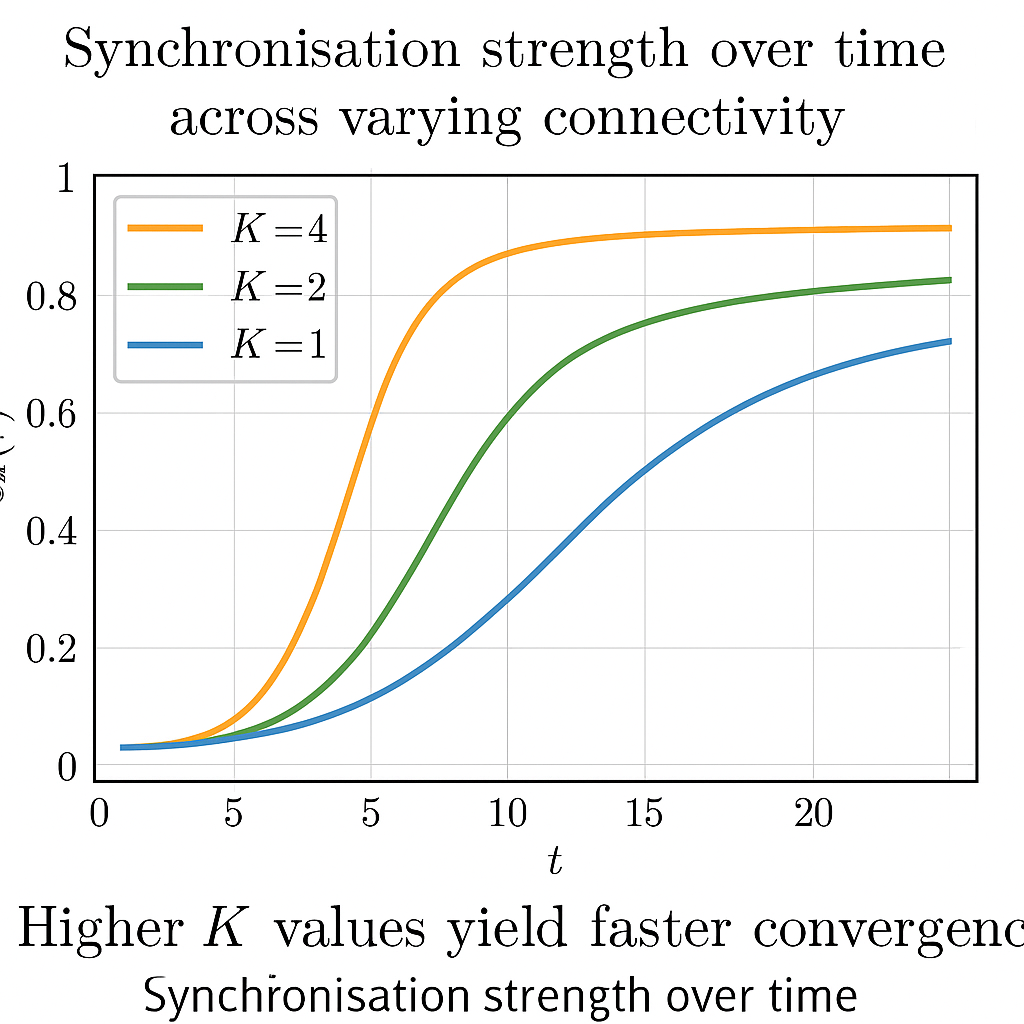
\includegraphics[width=0.7\linewidth]{sync_plot}
			\caption{Synchronisation strength over time across varying connectivity. Higher $K$ values yield faster convergence.}
			\label{fig:sync_plot}
		\end{figure}
		
		\subsection{Noise Tolerance and Phase Drift}
		\lipsum[5]
		
		\subsection{Synchrony Breakdown}
		Under strong environmental perturbations (modeled as phase noise), synchrony collapses but recovers if agents adapt their coupling strength.
		
		\section{Discussion}
		\lipsum[6-7]
		
		This model highlights the resilience and fragility of synchrony \cite{grinsteinSteeredResponsePower2024, jensArrayvolutionUsingMicrophone, nehoraiAcousticVectorsensorArray1994, spiesbergerHyperbolicLocationErrors2001b, wajidDesignAnalysisAir2016} in collective systems. Possible applications include swarm robotics, synthetic neural circuits, and network optimisation.
		
		\section{Conclusion}
		\Our{} computational model of synchrony provides new insights into collective coordination. Future work could extend this to dynamic topology, feedback-based coupling, or real-world robotic implementations.
		
	\end{maintext}
	
	% ------------------- Footer Manuscript Info -------------------
	\greyhrule
	\begin{manuscriptinfo}
	\end{manuscriptinfo}
	
	% ------------------- Bibliography -------------------
	\greyhrule
	\printbibliography
	
\end{document}